% Options for packages loaded elsewhere
% Options for packages loaded elsewhere
\PassOptionsToPackage{unicode}{hyperref}
\PassOptionsToPackage{hyphens}{url}
\PassOptionsToPackage{dvipsnames,svgnames,x11names}{xcolor}
%
\documentclass[
  letterpaper,
  DIV=11,
  numbers=noendperiod]{scrartcl}
\usepackage{xcolor}
\usepackage{amsmath,amssymb}
\setcounter{secnumdepth}{-\maxdimen} % remove section numbering
\usepackage{iftex}
\ifPDFTeX
  \usepackage[T1]{fontenc}
  \usepackage[utf8]{inputenc}
  \usepackage{textcomp} % provide euro and other symbols
\else % if luatex or xetex
  \usepackage{unicode-math} % this also loads fontspec
  \defaultfontfeatures{Scale=MatchLowercase}
  \defaultfontfeatures[\rmfamily]{Ligatures=TeX,Scale=1}
\fi
\usepackage{lmodern}
\ifPDFTeX\else
  % xetex/luatex font selection
\fi
% Use upquote if available, for straight quotes in verbatim environments
\IfFileExists{upquote.sty}{\usepackage{upquote}}{}
\IfFileExists{microtype.sty}{% use microtype if available
  \usepackage[]{microtype}
  \UseMicrotypeSet[protrusion]{basicmath} % disable protrusion for tt fonts
}{}
\makeatletter
\@ifundefined{KOMAClassName}{% if non-KOMA class
  \IfFileExists{parskip.sty}{%
    \usepackage{parskip}
  }{% else
    \setlength{\parindent}{0pt}
    \setlength{\parskip}{6pt plus 2pt minus 1pt}}
}{% if KOMA class
  \KOMAoptions{parskip=half}}
\makeatother
% Make \paragraph and \subparagraph free-standing
\makeatletter
\ifx\paragraph\undefined\else
  \let\oldparagraph\paragraph
  \renewcommand{\paragraph}{
    \@ifstar
      \xxxParagraphStar
      \xxxParagraphNoStar
  }
  \newcommand{\xxxParagraphStar}[1]{\oldparagraph*{#1}\mbox{}}
  \newcommand{\xxxParagraphNoStar}[1]{\oldparagraph{#1}\mbox{}}
\fi
\ifx\subparagraph\undefined\else
  \let\oldsubparagraph\subparagraph
  \renewcommand{\subparagraph}{
    \@ifstar
      \xxxSubParagraphStar
      \xxxSubParagraphNoStar
  }
  \newcommand{\xxxSubParagraphStar}[1]{\oldsubparagraph*{#1}\mbox{}}
  \newcommand{\xxxSubParagraphNoStar}[1]{\oldsubparagraph{#1}\mbox{}}
\fi
\makeatother


\usepackage{longtable,booktabs,array}
\usepackage{calc} % for calculating minipage widths
% Correct order of tables after \paragraph or \subparagraph
\usepackage{etoolbox}
\makeatletter
\patchcmd\longtable{\par}{\if@noskipsec\mbox{}\fi\par}{}{}
\makeatother
% Allow footnotes in longtable head/foot
\IfFileExists{footnotehyper.sty}{\usepackage{footnotehyper}}{\usepackage{footnote}}
\makesavenoteenv{longtable}
\usepackage{graphicx}
\makeatletter
\newsavebox\pandoc@box
\newcommand*\pandocbounded[1]{% scales image to fit in text height/width
  \sbox\pandoc@box{#1}%
  \Gscale@div\@tempa{\textheight}{\dimexpr\ht\pandoc@box+\dp\pandoc@box\relax}%
  \Gscale@div\@tempb{\linewidth}{\wd\pandoc@box}%
  \ifdim\@tempb\p@<\@tempa\p@\let\@tempa\@tempb\fi% select the smaller of both
  \ifdim\@tempa\p@<\p@\scalebox{\@tempa}{\usebox\pandoc@box}%
  \else\usebox{\pandoc@box}%
  \fi%
}
% Set default figure placement to htbp
\def\fps@figure{htbp}
\makeatother





\setlength{\emergencystretch}{3em} % prevent overfull lines

\providecommand{\tightlist}{%
  \setlength{\itemsep}{0pt}\setlength{\parskip}{0pt}}



 


\KOMAoption{captions}{tableheading}
\makeatletter
\@ifpackageloaded{caption}{}{\usepackage{caption}}
\AtBeginDocument{%
\ifdefined\contentsname
  \renewcommand*\contentsname{Table of contents}
\else
  \newcommand\contentsname{Table of contents}
\fi
\ifdefined\listfigurename
  \renewcommand*\listfigurename{List of Figures}
\else
  \newcommand\listfigurename{List of Figures}
\fi
\ifdefined\listtablename
  \renewcommand*\listtablename{List of Tables}
\else
  \newcommand\listtablename{List of Tables}
\fi
\ifdefined\figurename
  \renewcommand*\figurename{Figure}
\else
  \newcommand\figurename{Figure}
\fi
\ifdefined\tablename
  \renewcommand*\tablename{Table}
\else
  \newcommand\tablename{Table}
\fi
}
\@ifpackageloaded{float}{}{\usepackage{float}}
\floatstyle{ruled}
\@ifundefined{c@chapter}{\newfloat{codelisting}{h}{lop}}{\newfloat{codelisting}{h}{lop}[chapter]}
\floatname{codelisting}{Listing}
\newcommand*\listoflistings{\listof{codelisting}{List of Listings}}
\makeatother
\makeatletter
\makeatother
\makeatletter
\@ifpackageloaded{caption}{}{\usepackage{caption}}
\@ifpackageloaded{subcaption}{}{\usepackage{subcaption}}
\makeatother
\usepackage{bookmark}
\IfFileExists{xurl.sty}{\usepackage{xurl}}{} % add URL line breaks if available
\urlstyle{same}
\hypersetup{
  pdftitle={Hakkımda},
  colorlinks=true,
  linkcolor={blue},
  filecolor={Maroon},
  citecolor={Blue},
  urlcolor={Blue},
  pdfcreator={LaTeX via pandoc}}


\title{Hakkımda}
\author{}
\date{}
\begin{document}
\maketitle


\begin{center}
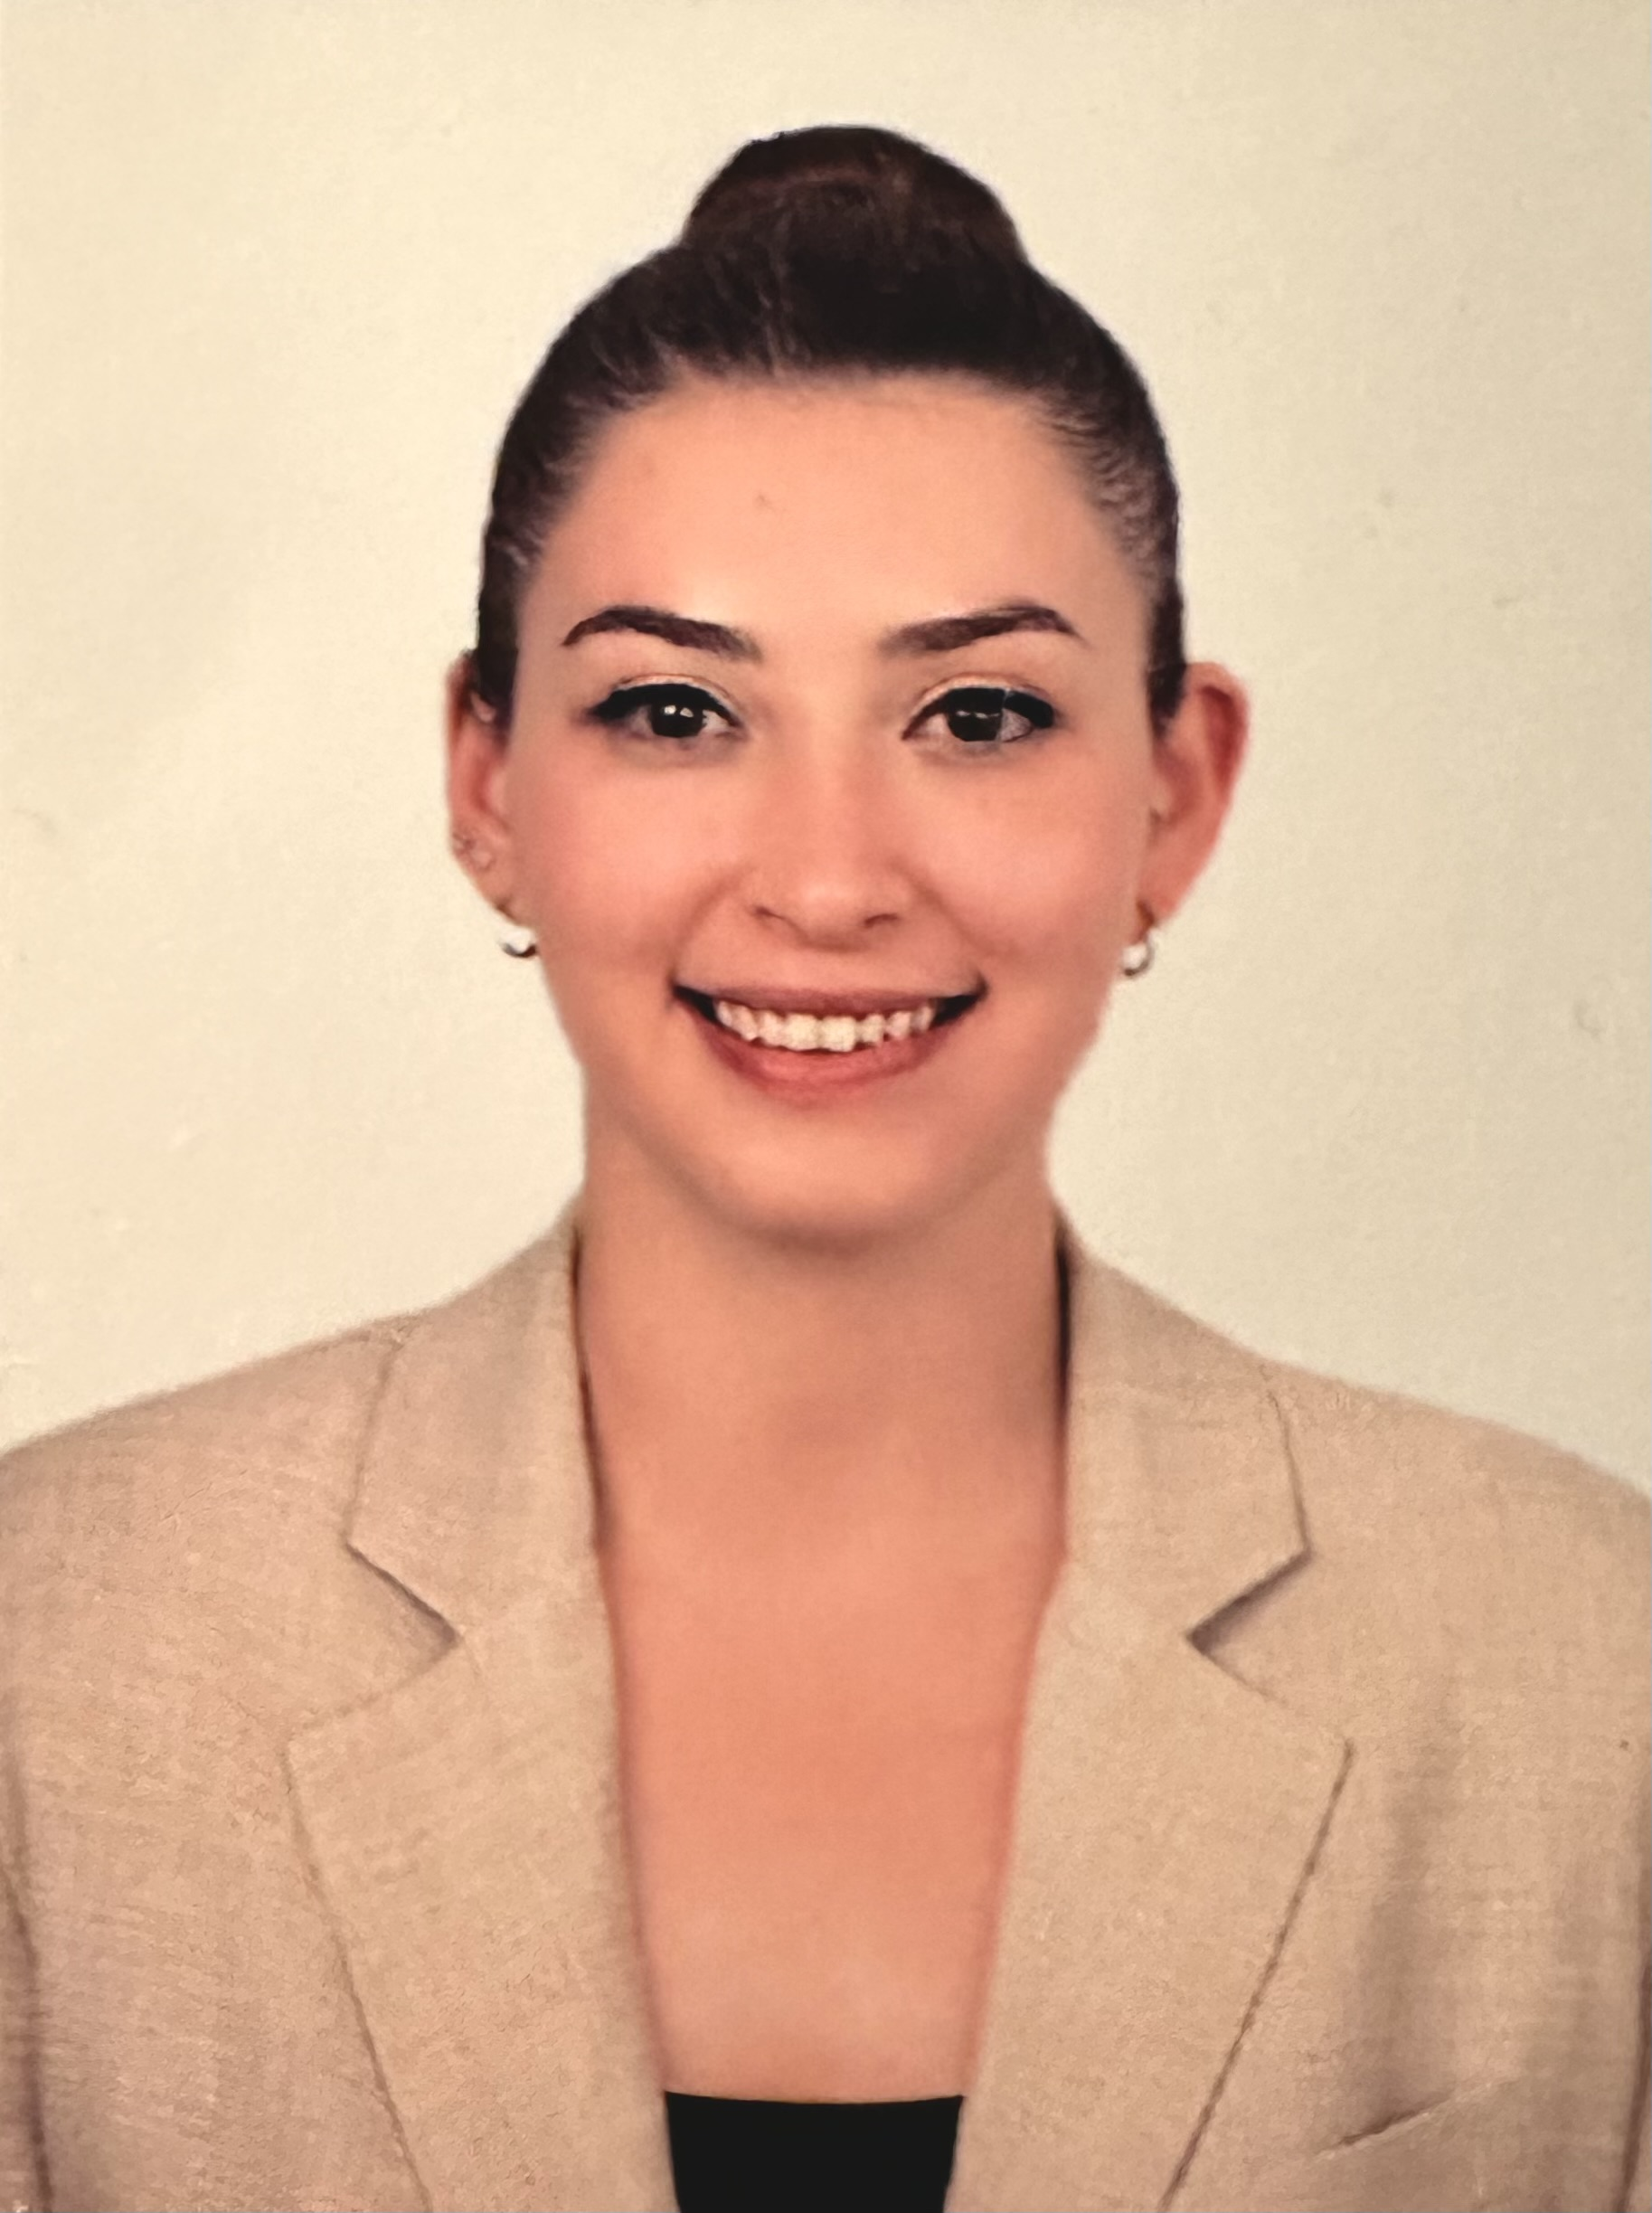
\includegraphics[width=2.34375in,height=\textheight,keepaspectratio]{images/IMG_6584.jpg}
\end{center}

\section{Eğitim}\label{eux11fitim}

\begin{itemize}
\tightlist
\item
  Yüksek Lisans, Mühendislik Yönetimi, Hacettepe Üniversitesi, 2026 -
  Devam Ediyor
\item
  Lisans, İktisat, Uludağ Üniversitesi, 2013 - 2018
\end{itemize}

\section{Deneyimler}\label{deneyimler}

\subsection{İş Tecrübesi}\label{iux15f-tecruxfcbesi}

\begin{itemize}
\item
  \textbf{Megart Teknoloji San. Tic. A.Ş.}

  Üretim Planlama ve Satın Alma Müdürü (Ekim 2025 - Devam Ediyor)Satın
  Alma Uzmanı (Ağustos 2023 - Ekim 2025)
\item
  \textbf{Mebant İzolasyon ve Bant San. A.Ş.}

  Sistem ve Süreç Geliştirme Yöneticisi (Ocak 2023 - Ağustos 2023)Sistem
  ve Süreç Geliştirme Uzmanı (Kasım 2021 - Aralık 2022)
\item
  \textbf{Billas Lastik ve Kauçuk San. Tic. A.Ş.}

  Kalite Yönetim Sistemleri Sorumlusu (Eylül 2018 - Kasım 2021
\end{itemize}

\subsection{Stajlar}\label{stajlar}

\begin{itemize}
\item
  \textbf{Türk Pirelli Lastikleri A.Ş.}

  İnsan Kaynakları Stajyeri (Ağustos 2016 - Eylül 2016)
\end{itemize}

\section{Sertifikalar}\label{sertifikalar}

\begin{itemize}
\item
  \textbf{MMOG/LE V.6} Ford Motor Company
\item
  \textbf{IATF 16949:2016 Otomotiv Kalite Yönetim Sistemleri --
  Bilgilendirme Eğitimi} (Sertifika No: 2023028) -- Redline Denetim \&
  Eğitim Hizmetleri
\item
  \textbf{ISO 19011 İç Tetkikçi Sertifikası} (Sertifika No: 2023048) --
  Redline Denetim \& Eğitim Hizmetleri
\item
  \textbf{AIAG \& VDA FMEA V1} (Sertifika No: 2023001) -- Redline
  Denetim \& Eğitim Hizmetleri
\item
  \textbf{VDA 6.3 Proses İç Tetkikçisi \& VDA -- Alman Otomotiv KYS
  Bilinç Eğitimi} (Sertifika No: RIS25062022.02) -- Redline Denetim \&
  Eğitim Hizmetleri
\item
  \textbf{IATF 16949:2016 İPK Eğitimi (MSA 4th, SPC 2nd)} (Sertifika No:
  RIS26072022.02) -- Redline Denetim \& Eğitim Hizmetleri
\item
  \textbf{ISO 14001:2015 Çevre Yönetim Sistemleri -- Bilgilendirme
  Eğitimi} (Sertifika No: 40079) -- Gelişim Yönetim Sistemleri A.Ş.
\item
  \textbf{Sürdürülebilir Satın Alma}Demirci Eğitim \& Danışmanlık
\item
  \textbf{A'dan Z'ye Etkili İletişim} (Sertifika No: UC-YSB2O31W) --
  Udemy
\item
  \textbf{Kaizen -- Değişim ve Sürekli İyileştirme} (Sertifika No: 2866)
  -- Elginkan Vakfı
\end{itemize}

\section{Yetenekler}\label{yetenekler}

\begin{itemize}
\tightlist
\item
  Microsoft Office Programları (İleri Düzeyde)
\item
  Canias ERP
\item
  QDMS Entegre Yönetim Sistemleri
\item
  Freedom ERP
\item
  Altasoft E-FMEA
\item
  CoralReef MES
\item
  Netsis
\item
  Problem Çözme Teknikleri (5Why, Ishikawa, 5N1K, Pareto)
\end{itemize}

\section{Projeler}\label{projeler}

\textbf{Canias ERP Devreye Alma Projesi}

\textbf{Proje Yöneticisi (Ağustos 2025 - Devam Ediyor)}

ERP sisteminin uçtan uca devreye alınması kapsamında temel veri, kalite,
satın alma ve envanter modüllerinin kurulumu ve süreç kurguları
yönetildi.

\emph{Temel Veri Yönetimi}

Malzeme kartlarının hammadde, yarı mamul, bitmiş ürün, sabit kıymet,
fason vb. olarak sınıflandırılmıştır. Malzemeler için minimum sipariş
miktarı, termin süresi, minimum güvenlik stoğu, kalite planları vb.
kritik parametreler belirlenmiştir. Konfigürasyon ve revizyon takibi
için kodlama kurgusunun yapılmıştır. Fason, yarı mamül ve bitmiş ürün
BOM kurgusunun oluşturulmuştur. İş merkezi, üretim / montaj
operasyonlarının ve fason operasyonlar tanımlanmıştır. Oluşturulan iş
merkezleri ve operasyonlar ile rota girme sürecinin kurgulanmıştır.

📍Kazanımlar: Veri standardizasyonu sağlanarak süreçler içerisinde doğru
veri kaynağı oluşturulmuştur.

\emph{Kalite Yönetimi}

Hammaddeler için kalite kontrol planları, kontrol sıklıkları
oluşturulmuştur. GKK sürecinde kontrollerin EPR üzerinden yapılması
kurgulanmıştır. Yarı mamul ve bitmiş ürünler için ara ve final kalite
planları tanımlanmıştır. Değişiklik yönetiminin ERP'den yapılabilmesi
için BPM süreci kurgulanmıştır. Uygunsuzluk kayıtları için düzeltici
faaliyet süreci kurgulanmıştır.

📍Kazanımlar: Kalite kayıtlarının arşivlenmesi ve kalite sürecinde
izlenmebilirlik, eskalasyon sağlanmıştır.

\emph{Satınalma Yönetimi Modülü}

Talep , teklif, sipariş kurgusunun oluşturulmuştur. Fason siparişler ile
fason izlenebilirliği sağlanmıştır.

📍Kazanımlar: Tedarikçi performans değerlendirme süreci için zamanında
teslimat performası ve kalite performansı otomatik hesaplanabilmektedir.
Fason süreçlerde izlenebilirllik sağlanmıştır.

\emph{Envanter Yönetimi Modülü}

Depo ve stok lokasyon yapısı oluşturulmuştır. Proje bazlı stok tutma
senaryosundan malzeme bazlı stok tutma ve rezervasyon sistemine
geçilmiştir. Raf ömürlü malzemelerde raf ömrü ERP'ye entegre edilmiştir.
Güvenlik stoğu kontrolleri kurgusu yapılmıştır.

📍Kazanımlar: Stok doğruluğu artırıldı ve stok yönetimi optimize
edilmiştir.

Başlık




\end{document}
